\chapter{La stéréochimie approfondie}\label{ch:b1:stereochemistry-in-depth}

Écrasons quelques graines de carvi, puis une feuille de menthe verte~:
deux odeurs bien différentes. L'odorant principal de chacune est la
carvone, \ce{C10H14O}, avec les mêmes atomes liés dans le même ordre ---
mais les deux carvones sont images l'une de l'autre dans un miroir, comme
une main gauche l'est d'une main droite, et les récepteurs du nez,
eux-mêmes formés de molécules dépourvues de symétrie miroir, les
distinguent. Les médicaments, les arômes et les molécules du vivant sont
tous construits en trois dimensions, et une formule développée qui ignore
la troisième dimension manque la moitié de l'histoire. Ce chapitre donne
les outils pour dessiner les molécules dans l'espace, nommer chaque
arrangement sans ambiguïté, suivre les rotations que les molécules
effectuent sans cesse, et mesurer la seule propriété physique qui
distingue deux images miroir.

\begin{recall}
Le volume scolaire (année 12) a introduit les molécules \omterm{def:b1:stereochemistry-in-depth:stereocentre}{chirales}, le
carbone asymétrique, les \omterm{def:b1:stereochemistry-in-depth:enantiomers}{énantiomères}, les isomères $Z$/$E$ et les
\omterm{def:b1:stereochemistry-in-depth:isomers}{conformations} de l'éthane. La disposition tétraédrique de quatre liaisons
autour du carbone et la description $\sigma$/$\pi$ des liaisons simples
et doubles viennent du \cref{ch:b1:lewis-resonance-vsepr}.
\end{recall}

\begin{omfigure}
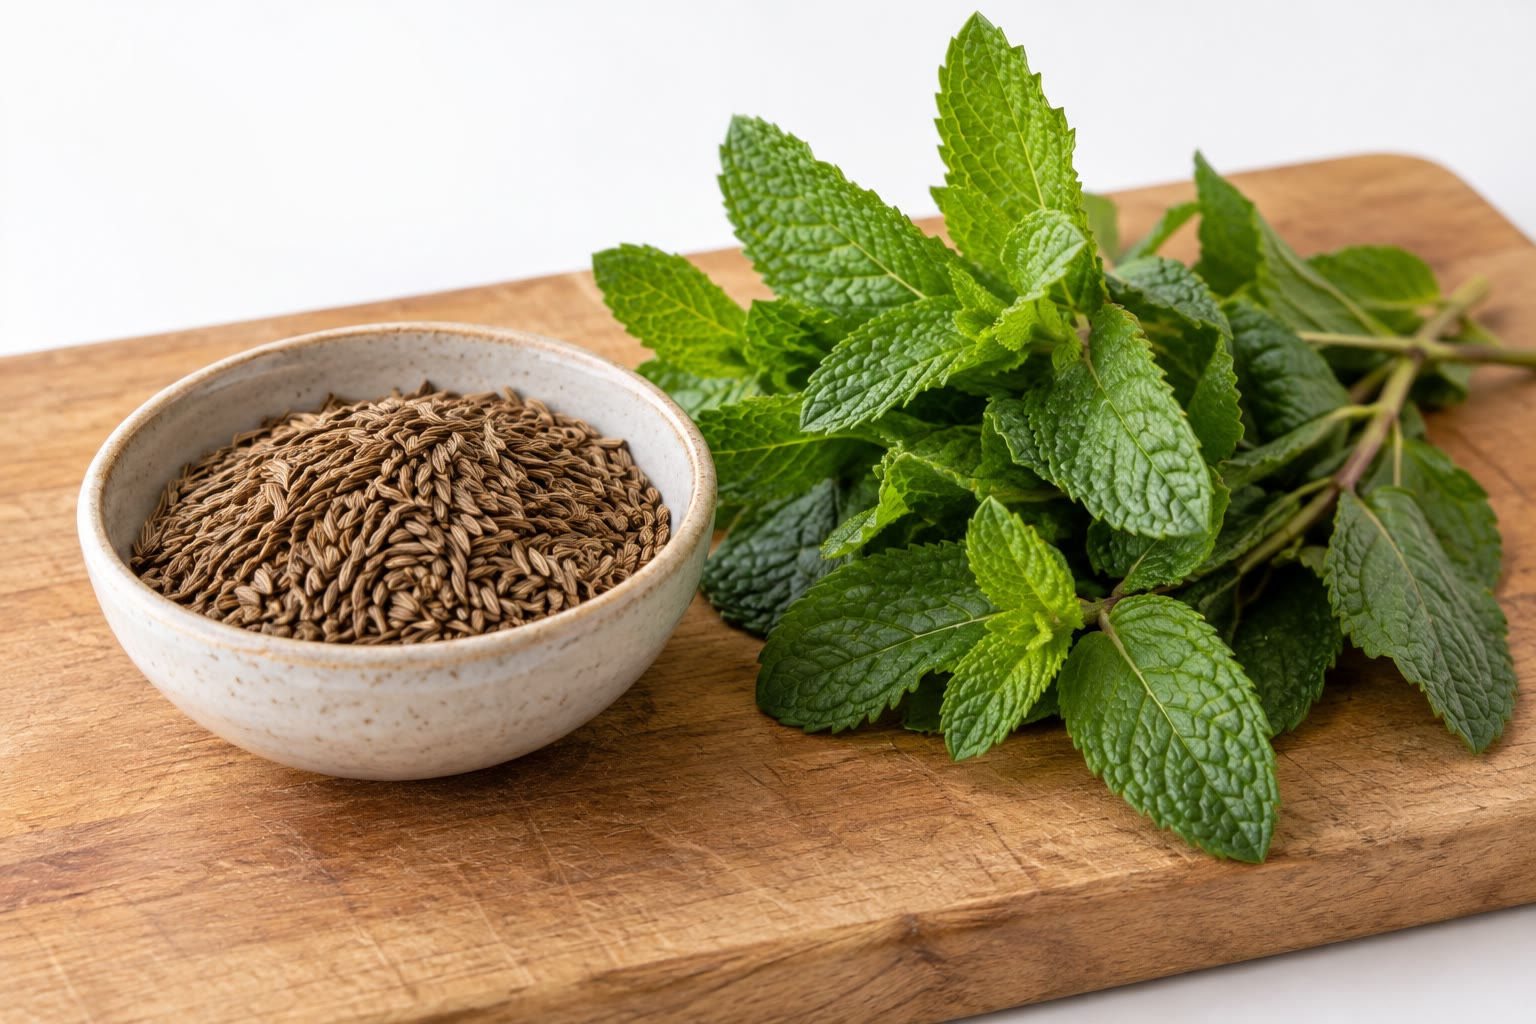
\includegraphics[width=0.55\linewidth]{images/book2/ai/b1-16-caraway-mint.jpg}

{\small Graines de carvi et feuilles de menthe verte. Le carvi doit son
odeur surtout à la \cip{S}-carvone, la menthe verte à son image miroir,
la \cip{R}-carvone.}
\end{omfigure}

\section{Isomères et représentations}

\begin{definition}[Constitution, configuration, conformation]\label{def:b1:stereochemistry-in-depth:isomers}
Deux composés de même formule dont les atomes sont liés dans un ordre
différent sont des \emph{isomères de constitution}\index{isomeres de constitution@isomères de constitution}. Des
composés de même constitution dont les atomes ne diffèrent que par leur
disposition dans l'espace sont des \emph{stéréoisomères}\index{stereoisomeres@stéréoisomères}. La
disposition qu'on ne peut modifier qu'en rompant des liaisons est la
\emph{configuration}\index{configuration} d'un stéréoisomère~; une
disposition obtenue par rotation autour de liaisons simples, sans en
rompre aucune, est une \emph{conformation}\index{conformation}.
\end{definition}

À température ambiante, les rotations autour des liaisons simples se
produisent des milliards de fois par seconde~: les \omterm{def:b1:stereochemistry-in-depth:isomers}{conformations}
s'interconvertissent et ne peuvent pas être isolées, tandis que les
\omterm{def:b1:stereochemistry-in-depth:isomers}{configurations} sont stables et donnent des composés distincts.

\begin{definition}[Représentations]\label{def:b1:stereochemistry-in-depth:representations}
Dans la \emph{représentation de Cram}\index{representation de Cram@représentation de Cram}, deux liaisons
sont dessinées dans le plan de la page, un coin plein pointe vers le
lecteur et un coin hachuré s'en éloigne. Une \emph{projection de
Newman}\index{projection de Newman} regarde une molécule le long d'une
liaison C--C~: le carbone avant est un point où se rejoignent ses trois
autres liaisons, le carbone arrière un cercle du bord duquel partent ses
liaisons. Dans une \emph{projection de Fischer}\index{projection de Fischer},
la chaîne carbonée est verticale, les liaisons horizontales pointent vers
le lecteur et les liaisons verticales s'en éloignent~; chaque croisement
est un carbone stéréogène.
\end{definition}

\begin{omfigure}
\begin{tikzpicture}[font=\small]
  % staggered and eclipsed ethane, Newman
  \pic (s) at (0,0) {omnewman={90}{30}};
  \foreach \k in {1,2,3} { \node at (s-f\k) {H}; \node at (s-b\k) {H}; }
  \node at (0,-1.9) {décalée};
  \pic (e) at (3.6,0) {omnewman={90}{108}};
  \foreach \k in {1,2,3} { \node at (e-f\k) {H}; }
  \foreach \k in {1,2,3} { \node[font=\scriptsize, black!60] at ($(e-b\k)!-0.12!(e-c)$) {H}; }
  \node at (3.6,-1.9) {éclipsée};
  % Fischer projection of (R)-lactic acid
  \begin{scope}[xshift=7.6cm]
    \draw[thick] (-0.9,0) -- (0.9,0) (0,-0.9) -- (0,0.9);
    \node[above] at (0,0.9) {\ce{COOH}};
    \node[below] at (0,-0.9) {\ce{CH3}};
    \node[left] at (-0.9,0) {H};
    \node[right] at (0.9,0) {OH};
    \node at (0,-1.9) {Fischer};
  \end{scope}
  % Cram of the same
  \begin{scope}[xshift=11.0cm]
    \node at (0,0) {\chemfig{C(-[2]COOH)(-[:210]H_3C)(<:[:-12]OH)(<[:-55]H)}};
    \node at (0,-1.9) {Cram};
  \end{scope}
\end{tikzpicture}

{\small À gauche~: \omterm{def:b1:stereochemistry-in-depth:representations}{projections de Newman} de l'éthane le long de sa
liaison C--C, en \omterm{def:b1:stereochemistry-in-depth:conformations}{conformation décalée} (liaisons arrière entre les
liaisons avant) et éclipsée (liaisons arrière cachées derrière les
liaisons avant, dessinées légèrement décalées). À droite~: la même
molécule, l'acide \cip{R}-lactique, en \omterm{def:b1:stereochemistry-in-depth:representations}{projection de Fischer} et en
\omterm{def:b1:stereochemistry-in-depth:representations}{représentation de Cram} (les liaisons verticales de la croix de Fischer
s'éloignent du lecteur, les horizontales pointent vers lui).}
\end{omfigure}

\begin{method}[De Cram à Newman]\label{met:b1:stereochemistry-in-depth:newman-from-cram}
\begin{enumerate}
  \item Choisir la liaison le long de laquelle on regarde et l'extrémité
        la plus proche de l'œil.
  \item Dessiner les trois liaisons du carbone avant à partir du centre,
        en conservant leur ordre (sens horaire ou antihoraire) tel que
        l'œil le voit.
  \item Dessiner les liaisons du carbone arrière à partir du cercle, dans
        l'ordre où on les voit du même côté.
  \item Vérifier~: tourner le carbone arrière de $60^\circ$ fait passer
        de la \omterm{def:b1:stereochemistry-in-depth:conformations}{conformation décalée} à l'éclipsée~; de $120^\circ$, d'une
        \omterm{def:b1:stereochemistry-in-depth:conformations}{conformation décalée} à la suivante.
\end{enumerate}
\end{method}

\section{Configuration~: les règles CIP}

\begin{definition}[Règles CIP, descripteurs]\label{def:b1:stereochemistry-in-depth:cip}
Les \emph{règles CIP}\index{regles CIP@règles CIP} (Cahn--Ingold--Prelog) classent les
quatre substituants d'un \omterm{def:b1:stereochemistry-in-depth:stereocentre}{centre stéréogène}~: le numéro atomique le plus
élevé d'abord~; en cas d'égalité, on compare les ensembles d'atomes
attachés au rang suivant, et ainsi de suite vers l'extérieur~; une
liaison double compte comme deux liaisons simples vers des atomes
dupliqués. Le substituant de plus bas rang étant dirigé à l'opposé de
l'œil, la séquence
$1 \to 2 \to 3$ tournant dans le sens horaire définit le descripteur
\cip{R}, et dans le sens antihoraire \cip{S}. Pour une liaison double
portant deux substituants sur chaque carbone, \cip{Z} signifie que les
deux substituants de plus haut rang sont du même côté, et \cip{E} qu'ils
sont de part et d'autre.
\end{definition}

\begin{method}[Attribuer \texorpdfstring{\cip{R}}{(R)} ou \texorpdfstring{\cip{S}}{(S)}]\label{met:b1:stereochemistry-in-depth:cip}
\begin{enumerate}
  \item Classer les quatre substituants par les \omterm{def:b1:stereochemistry-in-depth:cip}{règles CIP}.
  \item Si le substituant de plus bas rang s'éloigne de vous (coin
        hachuré, ou liaison verticale d'une \omterm{def:b1:stereochemistry-in-depth:representations}{projection de Fischer}), lire
        directement le sens de rotation de $1 \to 2 \to 3$.
  \item S'il pointe vers vous (coin plein, liaison horizontale de
        Fischer), lire le sens de rotation et inverser le descripteur.
  \item Échanger deux substituants quelconques inverse le descripteur~:
        c'est une vérification rapide.
\end{enumerate}
Dans l'acide lactique, $\ce{OH} > \ce{COOH} > \ce{CH3} > \ce{H}$ (O~;
puis C(O,O,O) l'emporte sur C(H,H,H)). Dans la \omterm{def:b1:stereochemistry-in-depth:representations}{projection de Fischer}
ci-dessus, H est horizontal (vers nous) et
$\ce{OH} \to \ce{COOH} \to \ce{CH3}$ tourne dans le sens antihoraire~:
en inversant, le centre est \cip{R}.
\end{method}

\section{La chiralité et ses conséquences}

\begin{definition}[Centre stéréogène, chiralité]\label{def:b1:stereochemistry-in-depth:stereocentre}
Un objet est \emph{chiral}\index{chiral} s'il n'est pas superposable à
son image dans un miroir, \emph{achiral}\index{achiral} sinon~; cette
propriété est la \emph{chiralité}\index{chiralite@chiralité}. Un \emph{centre
stéréogène}\index{centre stereogene@centre stéréogène} est un atome où l'échange de deux
substituants donne un stéréoisomère~; un carbone tétraédrique portant
quatre substituants différents en est un.
\end{definition}

Une molécule qui possède un plan de symétrie ou un centre de symétrie est
achirale~; une molécule qui n'a ni l'un ni l'autre est chirale en
pratique. Le critère exact, en termes d'opérations de symétrie, est donné
dans le volume de troisième année.

\begin{definition}[Énantiomères, diastéréoisomères, composé méso, mélange racémique]\label{def:b1:stereochemistry-in-depth:enantiomers}
Deux \omterm{def:b1:stereochemistry-in-depth:isomers}{stéréoisomères} images l'un de l'autre dans un miroir sont des
\emph{énantiomères}\index{enantiomeres@énantiomères}~; des \omterm{def:b1:stereochemistry-in-depth:isomers}{stéréoisomères} qui ne le sont pas sont
des \emph{diastéréoisomères}\index{diastereoisomeres@diastéréoisomères}. Un \emph{composé
méso}\index{compose meso@composé méso} possède des \omterm{def:b1:stereochemistry-in-depth:stereocentre}{centres stéréogènes} mais est \omterm{def:b1:stereochemistry-in-depth:stereocentre}{achiral}. Un
mélange équimolaire de deux énantiomères est un \emph{mélange
racémique}\index{melange racemique@mélange racémique}.
\end{definition}

\begin{proposition}[Nombre de stéréoisomères]\label{prop:b1:stereochemistry-in-depth:max-stereoisomers}
Une molécule possédant $n$ \omterm{def:b1:stereochemistry-in-depth:stereocentre}{centres stéréogènes} (et aucun autre élément
stéréogène) a au plus $2^n$ \omterm{def:b1:stereochemistry-in-depth:isomers}{stéréoisomères}, formant au plus $2^{n-1}$
couples d'\omterm{def:b1:stereochemistry-in-depth:enantiomers}{énantiomères}~; les formes méso réduisent ce nombre.
\end{proposition}

\begin{proof}
Chaque centre est \cip{R} ou \cip{S} indépendamment~: $2^n$
combinaisons. L'image miroir change chaque descripteur, si bien que les
combinaisons se regroupent par paires d'\omterm{def:b1:stereochemistry-in-depth:enantiomers}{énantiomères}, $2^{n-1}$ paires.
Si une combinaison est sa propre image miroir après une rotation de la
molécule (une forme méso), sa paire se réduit à un seul composé.
\end{proof}

L'acide tartrique, \ce{HOOC-CH(OH)-CH(OH)-COOH}, possède deux centres
équivalents~: \cip{R,R} et \cip{S,S} sont des \omterm{def:b1:stereochemistry-in-depth:enantiomers}{énantiomères}, tandis que
\cip{R,S} possède un plan de symétrie entre les deux carbones et est
méso~: trois \omterm{def:b1:stereochemistry-in-depth:isomers}{stéréoisomères}, et non quatre.

\begin{proposition}[Propriétés des énantiomères]\label{prop:b1:stereochemistry-in-depth:enantiomer-properties}
Deux \omterm{def:b1:stereochemistry-in-depth:enantiomers}{énantiomères} ont les mêmes températures de fusion et d'ébullition,
les mêmes \omterm{def:b1:precipitation:solubility}{solubilités} dans les solvants achiraux, les mêmes spectres et
la même réactivité vis-à-vis des réactifs achiraux~; ils diffèrent par
leur action sur la lumière polarisée et par leurs interactions avec
d'autres molécules \omterm{def:b1:stereochemistry-in-depth:stereocentre}{chirales}. Les \omterm{def:b1:stereochemistry-in-depth:enantiomers}{diastéréoisomères} diffèrent par toutes
leurs propriétés.
\end{proposition}

\begin{proof}
Toute propriété qui ne dépend que des distances et des angles à
l'intérieur de la molécule, ou entre celle-ci et des partenaires
achiraux, est la même pour un objet et son image miroir, puisqu'une
réflexion conserve les distances et les angles. Un partenaire \omterm{def:b1:stereochemistry-in-depth:stereocentre}{chiral} (un
récepteur, un réactif \omterm{def:b1:stereochemistry-in-depth:stereocentre}{chiral}, le trajet hélicoïdal de la lumière
polarisée décrit plus loin) forme des paires \omterm{def:b1:stereochemistry-in-depth:enantiomers}{diastéréoisomères}, qui ne
sont plus images l'une de l'autre et diffèrent donc. Les
\omterm{def:b1:stereochemistry-in-depth:enantiomers}{diastéréoisomères} ne sont reliés par aucune réflexion~: leurs distances
internes diffèrent.
\end{proof}

\begin{omfigure}
\begin{tikzpicture}[font=\small, line join=round]
  \foreach \dx/\kind/\lab in {0/1/{\cip{R}-carvone (menthe verte)}, 5.2/0/{\cip{S}-carvone (carvi)}} {
  \begin{scope}[xshift=\dx cm]
    \coordinate (c1) at (0,1); \coordinate (c2) at (0.87,0.5);
    \coordinate (c3) at (0.87,-0.5); \coordinate (c4) at (0,-1);
    \coordinate (c5) at (-0.87,-0.5); \coordinate (c6) at (-0.87,0.5);
    \draw[thick] (c1) -- (c2) -- (c3) -- (c4) -- (c5) -- (c6) -- cycle;
    \draw[thick] ($(c2)!0.15!(c3)+(-0.12,0)$) -- ($(c3)!0.15!(c2)+(-0.12,0)$);
    \draw[thick] (c1) -- ++(0,0.7) node[above] {O};
    \draw[thick] ($(c1)+(0.1,0)$) -- ++(0,0.62);
    \draw[thick] (c2) -- ++(0.75,0.43) node[right] {\ce{CH3}};
    \coordinate (q) at ($(c5)+(-0.75,-0.43)$);
    \ifnum\kind=1
      \fill (c5) -- ($(q)+(0.06,-0.1)$) -- ($(q)+(-0.06,0.1)$) -- cycle;
    \else
      \foreach \t in {0.15,0.3,0.45,0.6,0.75,0.9}
        \draw ($(c5)!\t!(q)+(\t*0.06,-\t*0.1)$) -- ($(c5)!\t!(q)+(-\t*0.06,\t*0.1)$);
    \fi
    \draw[thick] (q) -- ++(-0.6,0.5) node[above] {\ce{CH2}};
    \draw[thick] ($(q)+(0.08,0.06)$) -- ++(-0.6,0.5);
    \draw[thick] (q) -- ++(0,-0.75) node[below] {\ce{CH3}};
    \node[font=\scriptsize] at ($(c5)+(0.35,0.12)$) {5};
    \node at (0,-2.85) {\lab};
  \end{scope}}
\end{tikzpicture}

{\small Les deux carvones, dessinées sur le même squelette~: le groupe
isopropényle porté par C5 pointe vers le lecteur (coin plein) dans l'une
et s'éloigne du lecteur (coin hachuré) dans l'autre, l'hydrogène de C5
(non dessiné) étant du côté opposé. Elles sont images l'une de l'autre
dans un miroir~: ce sont des \omterm{def:b1:stereochemistry-in-depth:enantiomers}{énantiomères}
(\cref{exo:b1:stereochemistry-in-depth:4}).}
\end{omfigure}

\begin{history}[Un carbone tétraédrique]
\begin{minipage}[t]{0.2\linewidth}\vspace{0pt}
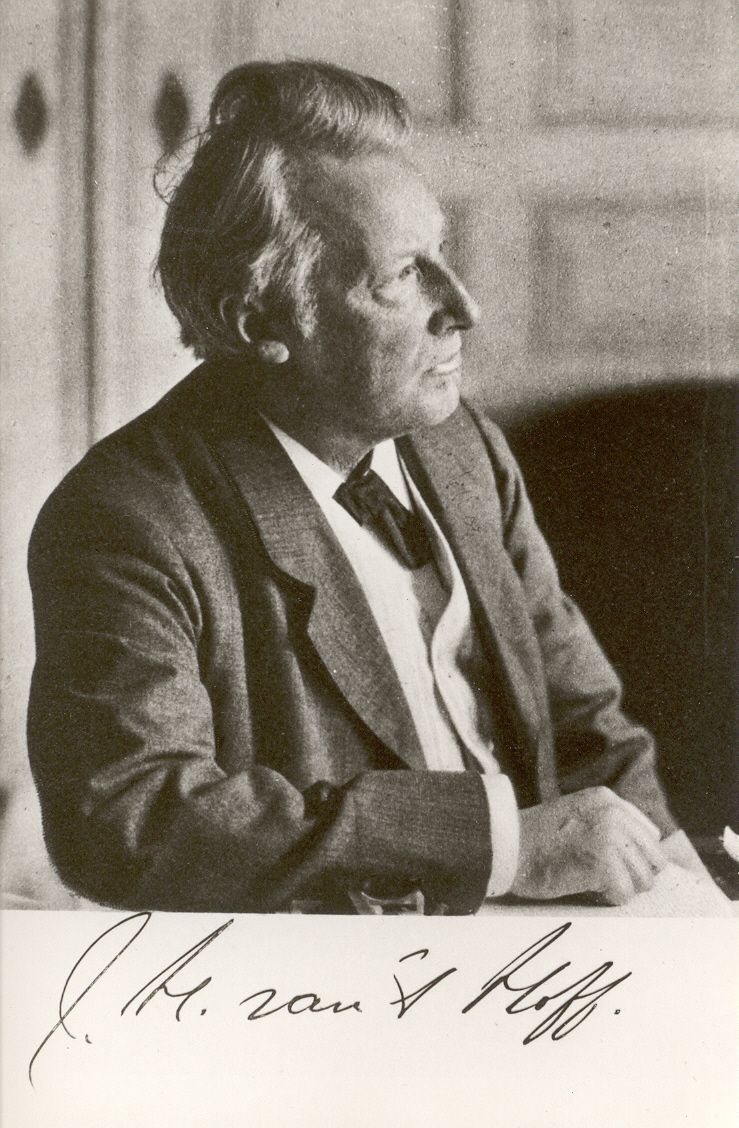
\includegraphics[width=\linewidth]{images/book2/van-t-hoff.jpg}
\end{minipage}\hfill
\begin{minipage}[t]{0.76\linewidth}\vspace{0pt}
Jacobus Henricus van 't Hoff proposa, jeune chimiste, que les quatre
liaisons d'un atome de carbone pointent vers les sommets d'un tétraèdre.
Un carbone portant quatre substituants différents existe alors sous deux
arrangements images l'un de l'autre, ce qui expliquait pourquoi certains
composés existent sous deux formes qui ne diffèrent que par le sens dans
lequel elles font tourner la lumière polarisée. Cette idée est le point
de départ de tous les dessins de ce chapitre. (Photographie publiée en
1911, domaine public, Wikimedia Commons.)
\end{minipage}
\end{history}

\section{Conformations}

\begin{definition}[Angle de torsion et conformations]\label{def:b1:stereochemistry-in-depth:conformations}
Pour quatre atomes A--B--C--D, l'\emph{angle de torsion}\index{angle de torsion}
$\theta$ autour de B--C est l'angle entre les plans ABC et BCD, lu sur
une \omterm{def:b1:stereochemistry-in-depth:representations}{projection de Newman} le long de B--C. Une \omterm{def:b1:stereochemistry-in-depth:isomers}{conformation} est une
\emph{conformation éclipsée}\index{conformation eclipsee@conformation éclipsée} lorsque les liaisons du carbone avant et
du carbone arrière sont alignées en projection, une \emph{conformation
décalée}\index{conformation decalee@conformation décalée} lorsqu'elles alternent. Dans le butane, vu le
long de C2--C3, la \omterm{def:b1:stereochemistry-in-depth:isomers}{conformation} décalée dont les deux groupes méthyle
sont à $180^\circ$ est la \emph{conformation anti}\index{conformation anti},
celles où ils sont à $\pm 60^\circ$ sont les \emph{conformations
gauches}\index{conformation gauche}. Dans le cyclohexane, le cycle
plissé sans tension est la \emph{chaise}\index{chaise}~; chaque carbone
porte une liaison \emph{axiale}\index{axiale}, parallèle à l'axe du
cycle, et une liaison \emph{équatoriale}\index{equatoriale@équatoriale}, à peu près dans le
plan moyen du cycle. L'\emph{inversion de chaise}\index{inversion de chaise} transforme une
chaise en l'autre, chaque liaison axiale devenant équatoriale et
inversement.
\end{definition}

\begin{omfigure}
\begin{tikzpicture}
\begin{axis}[
  width=0.82\linewidth, height=5.8cm, xmin=0, xmax=360, ymin=0, ymax=21,
  legend style={font=\scriptsize, draw=none, at={(0.5,0.62)}, anchor=center},
  axis x line=bottom, axis y line=left, xlabel={angle de torsion $\theta$ (degrés)},
  ylabel={énergie (kJ/mol)}, xtick={0,60,120,180,240,300,360},
  tick label style={font=\small}, label style={font=\small}]
\addplot[omDef, very thick] table[x=theta, y=butane] {figdata/out/bachelor-1-butane-torsion.dat};
\addplot[omProp, thick, dashed] table[x=theta, y=ethane] {figdata/out/bachelor-1-butane-torsion.dat};
\node[font=\scriptsize, anchor=south west] at (axis cs:0,18.4) {syn};
\node[font=\scriptsize, anchor=south] at (axis cs:62,18.4) {gauche};
\node[font=\scriptsize, anchor=south] at (axis cs:120,18.4) {éclipsée};
\node[font=\scriptsize, anchor=south] at (axis cs:180,18.4) {anti};
\node[font=\scriptsize, anchor=south] at (axis cs:240,18.4) {éclipsée};
\node[font=\scriptsize, anchor=south] at (axis cs:298,18.4) {gauche};
\node[font=\scriptsize, anchor=south east] at (axis cs:360,18.4) {syn};
\legend{butane, éthane}
\end{axis}
\end{tikzpicture}

{\small Énergie de torsion du butane autour de sa liaison centrale (trait
plein~; $\theta
= 0$ lorsque les groupes méthyle s'éclipsent) et de
l'éthane (tirets), calculées à partir de potentiels de torsion
expérimentaux. Éthane~: barrière de \qty{12.2}{kJ/mol}. Butane~: anti
le plus stable~; gauche \qty{2.8}{kJ/mol} plus haut, à
$\theta = 62^\circ$~; barrières de \qty{15.2}{kJ/mol} (méthyle éclipsant
un hydrogène) et de \qty{16.5}{kJ/mol} (méthyle éclipsant un méthyle).}
% ledger: rot:ethane-V3, rot:butane-V1, rot:butane-V2, rot:butane-V3, rot:butane-V4, rot:butane-V5, rot:butane-V6 (curves in figdata/bachelor-1/butane-torsion.py)
\end{omfigure}

Les barrières sont petites devant l'énergie thermique disponible lors
des chocs ($RT = \qty{2.5}{kJ/mol}$ à température ambiante, et bien
davantage dans la queue de la distribution,
\cref{ch:b1:elementary-steps})~: la rotation est rapide, et le butane est
un mélange de molécules anti et gauches qu'on ne peut pas séparer.

\begin{method}[Dessiner une chaise]\label{met:b1:stereochemistry-in-depth:draw-chair}
\begin{enumerate}
  \item Tracer deux traits parallèles légèrement inclinés vers le bas à
        droite, décalés~; joindre leurs extrémités par un V à gauche et
        par un V renversé à droite pour fermer le cycle à six atomes.
  \item Les liaisons \omterm{def:b1:stereochemistry-in-depth:conformations}{axiales} sont verticales~: vers le haut sur les
        carbones qui pointent vers le haut, vers le bas sur ceux qui
        pointent vers le bas, en alternance autour du cycle.
  \item Les liaisons \omterm{def:b1:stereochemistry-in-depth:conformations}{équatoriales} sont parallèles aux liaisons du cycle
        situées un rang plus loin, et pointent vers l'extérieur.
  \item Pour inverser le cycle, dessiner l'autre \omterm{def:b1:stereochemistry-in-depth:conformations}{chaise}~; un substituant
        \omterm{def:b1:stereochemistry-in-depth:conformations}{axial} dans l'une est \omterm{def:b1:stereochemistry-in-depth:conformations}{équatorial} dans l'autre.
\end{enumerate}
\end{method}

\begin{omfigure}
\begin{tikzpicture}[font=\small]
  \pic (a) at (0,0) {omchair};
  \foreach \k in {1,2,3,4,5,6} \draw[omProp, thick] (a-c\k) -- (a-a\k);
  \foreach \k in {1,2,3,4,5,6} \draw[omDef, thick] (a-c\k) -- (a-e\k);
  \node[omProp, anchor=south] at (a-a3) {axiale};
  \node[omDef, anchor=north] at (a-e5) {équatoriale};
  \begin{scope}[xshift=4.9cm]
    \pic (b) at (0,0) {omchair};
    \draw[thick] (b-c1) -- (b-e1) node[right] {\ce{CH3}};
    \draw[thick] (b-c1) -- (b-a1) node[above] {H};
    \node at (0,-1.5) {\ce{CH3} équatorial};
  \end{scope}
  \draw[<->, thick] (8.1,0) -- (8.8,0) node[midway, above] {inversion};
  \begin{scope}[xshift=10.45cm]
    \pic (c) at (0,0) {omchairflip};
    \draw[thick] (c-c4) -- (c-a4) node[below] {\ce{CH3}};
    \draw[thick] (c-c4) -- (c-e4) node[right] {H};
    \node at (0,-1.5) {\ce{CH3} axial};
  \end{scope}
\end{tikzpicture}

{\small À gauche~: la \omterm{def:b1:stereochemistry-in-depth:conformations}{chaise} du cyclohexane avec ses six liaisons
\omterm{def:b1:stereochemistry-in-depth:conformations}{axiales} (en orange, alternativement vers le haut et vers le bas) et ses
six liaisons \omterm{def:b1:stereochemistry-in-depth:conformations}{équatoriales} (en bleu). À droite~: les deux \omterm{def:b1:stereochemistry-in-depth:conformations}{chaises} du
méthylcyclohexane, interconverties par l'\omterm{def:b1:stereochemistry-in-depth:conformations}{inversion de chaise}~; le groupe
méthyle est \omterm{def:b1:stereochemistry-in-depth:conformations}{équatorial} dans l'une, \omterm{def:b1:stereochemistry-in-depth:conformations}{axial} dans l'autre.}
\end{omfigure}

\begin{proposition}[Les substituants équatoriaux sont préférés]\label{prop:b1:stereochemistry-in-depth:chair-substituent}
Dans un cyclohexane monosubstitué, la \omterm{def:b1:stereochemistry-in-depth:conformations}{chaise} où le substituant est
\omterm{def:b1:stereochemistry-in-depth:conformations}{équatorial} est la plus stable. Pour un groupe méthyle, la position
axiale ajoute deux interactions gauches avec des carbones du cycle,
valant chacune celle du butane (\qtyrange{2.8}{2.9}{kJ/mol}), soit
environ \qty{5.7}{kJ/mol} au total~: c'est une estimation de la
différence d'énergie.
\end{proposition}

\begin{proof}
Vu le long de la liaison C1--C2, un méthyle \omterm{def:b1:stereochemistry-in-depth:conformations}{axial} sur C1 est gauche par
rapport à C3 du cycle~; vu le long de C1--C6, gauche par rapport à C5~:
deux interactions gauches de type butane, qu'on voit aussi comme
l'encombrement du méthyle avec les hydrogènes \omterm{def:b1:stereochemistry-in-depth:conformations}{axiaux} portés par C3 et C5
(les interactions 1,3-diaxiales). Un méthyle \omterm{def:b1:stereochemistry-in-depth:conformations}{équatorial} est anti par
rapport à C3 et à C5. Chaque interaction gauche coûte ce qu'elle coûte
dans le butane, \qty{2.8}{kJ/mol} dans le potentiel de torsion de la
figure.
\end{proof}

Avec $\Delta E = \qty{5.7}{kJ/mol}$, le rapport des \omterm{def:b1:stereochemistry-in-depth:conformations}{chaises} \omterm{def:b1:stereochemistry-in-depth:conformations}{équatoriale}
et \omterm{def:b1:stereochemistry-in-depth:conformations}{axiale} à \qty{25}{\celsius} vaut $\exp(\Delta E/RT) = 10$~: environ
\qty{91}{\percent} de \omterm{def:b1:stereochemistry-in-depth:conformations}{chaises} \omterm{def:b1:stereochemistry-in-depth:conformations}{équatoriales}
(\cref{exo:b1:stereochemistry-in-depth:9}). Les groupes volumineux,
comme le groupe \textit{tert}-butyle, bloquent le cycle dans la \omterm{def:b1:stereochemistry-in-depth:conformations}{chaise} où
ils sont \omterm{def:b1:stereochemistry-in-depth:conformations}{équatoriaux}.

\section{L'activité optique}

\begin{definition}[Activité optique, pouvoir rotatoire spécifique]\label{def:b1:stereochemistry-in-depth:optical-activity}
Une substance présente une \emph{activité optique}\index{activite optique@activité optique} si elle
fait tourner le plan de polarisation d'une lumière polarisée
rectilignement qui la traverse. Pour un observateur placé face à la
lumière, une substance \emph{dextrogyre}\index{dextrogyre}, notée
$(+)$, le fait tourner dans le sens horaire, une substance
\emph{lévogyre}\index{levogyre@lévogyre}, notée $(-)$, dans le sens antihoraire. Le
\emph{pouvoir rotatoire spécifique}\index{pouvoir rotatoire specifique@pouvoir rotatoire spécifique} vaut
$[\alpha] = \alpha/(\ell c)$, où $\alpha$ est l'angle mesuré en degrés,
$\ell$ la longueur traversée en décimètres et $c$ la concentration
massique en \unit{g/mL}~; il dépend de la longueur d'onde (en général la
raie jaune du sodium), de la température et du solvant.
\end{definition}

\begin{omfigure}
\begin{tikzpicture}[font=\small, >={Stealth}]
  \fill[yellow!70!orange] (0,0) circle (0.25);
  \node[below] at (0,-0.45) {lampe};
  \draw[thick] (1.3,-0.7) rectangle (1.45,0.7); \node[below] at (1.37,-0.75) {polariseur};
  \draw[omDef!20, fill=omDef!10] (2.4,-0.45) rectangle (5.6,0.45);
  \node at (4.0,0) {échantillon, longueur $\ell$};
  \draw[thick] (6.5,-0.7) rectangle (6.65,0.7); \node[below] at (6.57,-0.75) {analyseur};
  \draw (7.6,0) circle (0.3); \node[below] at (7.6,-0.45) {œil};
  \draw[->, orange!80!black] (0.3,0) -- (1.25,0);
  \draw[->, orange!80!black] (1.5,0) -- (2.35,0);
  \draw[->, orange!80!black] (5.65,0) -- (6.45,0);
  % polarisation planes
  \draw[thick, omThm] (1.9,-0.35) -- (1.9,0.35);
  \draw[thick, omThm] (6.05,-0.33) -- ++(70:0.0) -- (5.93,0.33);
  \draw[->, omThm] (5.75,0.55) arc[start angle=100, end angle=70, radius=0.6];
  \node[omThm, above] at (6.1,0.75) {$\alpha$};
\end{tikzpicture}

{\small Un polarimètre. Le polariseur ne laisse passer que la lumière qui
vibre dans un plan~; l'échantillon \omterm{def:b1:stereochemistry-in-depth:stereocentre}{chiral} fait tourner ce plan de
$\alpha$~; on tourne l'analyseur jusqu'à éteindre de nouveau la lumière,
ce qui mesure $\alpha$.}
\end{omfigure}

\begin{proposition}[Loi de Biot]\label{prop:b1:stereochemistry-in-depth:biot}
Pour une solution diluée de plusieurs solutés optiquement actifs, l'angle
de rotation est additif, $\alpha = \ell\sum_i [\alpha]_i c_i$ (\emph{loi
de Biot}\index{loi de Biot}). Deux \omterm{def:b1:stereochemistry-in-depth:enantiomers}{énantiomères} ont des \omterm{def:b1:stereochemistry-in-depth:optical-activity}{pouvoirs
rotatoires spécifiques} opposés~; un \omterm{def:b1:stereochemistry-in-depth:enantiomers}{mélange racémique} ne fait pas
tourner la lumière.
\end{proposition}

\begin{proof}
Chaque soluté contribue indépendamment en solution diluée, en proportion
du nombre de molécules traversées, c'est-à-dire de $\ell c_i$~; c'est le
contenu expérimental de la loi. Une réflexion change le sens horaire en
sens antihoraire~: la molécule image fait tourner le plan d'un angle
opposé, et dans un \omterm{def:b1:stereochemistry-in-depth:enantiomers}{mélange racémique} les deux contributions
s'annulent.
\end{proof}

Pour un mélange de deux \omterm{def:b1:stereochemistry-in-depth:enantiomers}{énantiomères} de concentration totale $c$, la
fraction
$x$ de la forme $(-)$ donne $\alpha = \ell c[\alpha]_{(-)}(x - (1 - x)) =
\ell c[\alpha]_{(-)}(2x - 1)$~: mesurer $\alpha$ donne la composition.
Le pouvoir rotatoire n'est relié au descripteur par aucune règle
simple~: un composé \cip{R} peut être $(+)$ ou $(-)$~; la
\cip{R}-carvone de la menthe verte est \omterm{def:b1:stereochemistry-in-depth:optical-activity}{lévogyre}.

\section{Exercices}

\begin{exercise}[$\star$]\label{exo:b1:stereochemistry-in-depth:1}
Classer chaque paire en \omterm{def:b1:stereochemistry-in-depth:isomers}{isomères de constitution}, \omterm{def:b1:stereochemistry-in-depth:enantiomers}{énantiomères},
\omterm{def:b1:stereochemistry-in-depth:enantiomers}{diastéréoisomères} ou deux \omterm{def:b1:stereochemistry-in-depth:isomers}{conformations} d'un même composé~: butan-1-ol
et butan-2-ol~; \cip{R}- et \cip{S}-butan-2-ol~; \cip{Z}- et
\cip{E}-but-2-ène~; les \omterm{def:b1:stereochemistry-in-depth:conformations}{conformations anti} et gauche du butane~;
acides \cip{R,R}- et \cip{R,S}-tartrique.
\end{exercise}

\begin{exercise}[$\star$]\label{exo:b1:stereochemistry-in-depth:2}
Classer par les \omterm{def:b1:stereochemistry-in-depth:cip}{règles CIP}~: \ce{-OH}, \ce{-NH2}, \ce{-CH3}, \ce{-H}~;
puis \ce{-CH2OH}, \ce{-CHO}, \ce{-COOH}, \ce{-CH(CH3)2}~; puis \ce{-Cl},
\ce{-CH2Cl}, \ce{-CCl3}, \ce{-Br}.
\end{exercise}

\begin{exercise}[$\star$]\label{exo:b1:stereochemistry-in-depth:3}
Combien de \omterm{def:b1:stereochemistry-in-depth:isomers}{stéréoisomères} le 2,3-dichlorobutane, le
2-bromo-3-chlorobutane et le pentane-2,4-diol possèdent-ils~?
Identifier les formes méso.
\end{exercise}

\begin{exercise}[$\star$]\label{exo:b1:stereochemistry-in-depth:4}
Classer les quatre substituants du C5 de la carvone par les \omterm{def:b1:stereochemistry-in-depth:cip}{règles CIP}
et vérifier les descripteurs donnés sur la figure des deux carvones (coin
plein~: le groupe isopropényle vers le lecteur, H à l'opposé).
\end{exercise}

\begin{exercise}[$\star\star$]\label{exo:b1:stereochemistry-in-depth:5}
Dessiner les \omterm{def:b1:stereochemistry-in-depth:representations}{projections de Newman} du butane le long de C2--C3 pour
$\theta = 0$, 60, 120 et $180^\circ$ et lire leurs énergies sur la
courbe. Quelle fraction des molécules serait gauche si les énergies des
\omterm{def:b1:stereochemistry-in-depth:conformations}{conformations gauche} et anti étaient égales~?
\end{exercise}

\begin{exercise}[$\star\star$]\label{exo:b1:stereochemistry-in-depth:6}
Dessiner la \omterm{def:b1:stereochemistry-in-depth:representations}{projection de Fischer} de la \cip{S}-alanine,
\ce{H2N-CH(CH3)-COOH}, le groupe acide en haut. De quel côté se trouve le
groupe amino~?
\end{exercise}

\begin{exercise}[$\star\star$]\label{exo:b1:stereochemistry-in-depth:7}
Montrer que le \textit{cis}-1,2-diméthylcyclohexane a un méthyle \omterm{def:b1:stereochemistry-in-depth:conformations}{axial}
et un \omterm{def:b1:stereochemistry-in-depth:conformations}{équatorial} dans ses deux \omterm{def:b1:stereochemistry-in-depth:conformations}{chaises}, alors que l'isomère
\textit{trans} possède une \omterm{def:b1:stereochemistry-in-depth:conformations}{chaise} où les deux sont \omterm{def:b1:stereochemistry-in-depth:conformations}{équatoriaux}. Quel
isomère est le plus stable~? Utiliser l'estimation du chapitre.
\end{exercise}

\begin{exercise}[$\star\star$]\label{exo:b1:stereochemistry-in-depth:8}
Une solution d'un composé \omterm{def:b1:stereochemistry-in-depth:stereocentre}{chiral} à \qty{0.100}{g/mL} dans un tube de
\qty{2.00}{dm} fait tourner la lumière de $+13.2^\circ$. Calculer
$[\alpha]$. Que donnerait un tube de
\qty{1.00}{dm}~? Et l'énantiomère à la même concentration~?
\end{exercise}

\begin{exercise}[$\star\star$]\label{exo:b1:stereochemistry-in-depth:9}
Calculer, avec $\Delta E = \qty{5.7}{kJ/mol}$ et le rapport de Boltzmann
$\exp(\Delta E/RT)$, la fraction des \omterm{def:b1:stereochemistry-in-depth:conformations}{chaises} du méthylcyclohexane à
méthyle \omterm{def:b1:stereochemistry-in-depth:conformations}{équatorial} à \qty{25}{\celsius} et à \qty{-50}{\celsius}.
\end{exercise}

\begin{exercise}[$\star\star\star$]\label{exo:b1:stereochemistry-in-depth:10}
Expliquer pourquoi l'éthane n'a qu'une sorte de \omterm{def:b1:stereochemistry-in-depth:conformations}{conformation décalée} et
le butane deux (anti et gauche), et pourquoi la \omterm{def:b1:stereochemistry-in-depth:conformations}{conformation gauche} est
moins stable. À l'aide des énergies de la figure, estimer le rapport des
populations anti : gauche du butane à \qty{25}{\celsius} (deux
\omterm{def:b1:stereochemistry-in-depth:conformations}{conformations gauches}, une anti).
\end{exercise}

\begin{exercise}[$\star\star\star$]\label{exo:b1:stereochemistry-in-depth:11}
On considère l'acide 2,3,4-trihydroxypentanedioïque,
\ce{HOOC-CH(OH)-CH(OH)-CH(OH)-COOH}. Compter ses \omterm{def:b1:stereochemistry-in-depth:stereocentre}{centres stéréogènes},
montrer que le carbone central n'est stéréogène que lorsque les deux
carbones extérieurs ont des descripteurs opposés (pseudo-asymétrique),
et compter les \omterm{def:b1:stereochemistry-in-depth:isomers}{stéréoisomères} (formes méso comprises).
\end{exercise}

\begin{exercise}[$\star\star\star$]\label{exo:b1:stereochemistry-in-depth:12}
Un échantillon d'un des \omterm{def:b1:stereochemistry-in-depth:enantiomers}{énantiomères} d'un composé
($[\alpha] = +66.0^\circ$ pour le composé pur dans les conditions utilisées) s'est
partiellement racémisé~: à \qty{0.050}{g/mL} dans un tube de
\qty{1.00}{dm}, il donne $+2.31^\circ$. Calculer les fractions des deux
\omterm{def:b1:stereochemistry-in-depth:enantiomers}{énantiomères}.
\end{exercise}

\section{Problème~: le menthol, la molécule qui rafraîchit}

\begin{problem}[{Problème du week-end --- les trois centres stéréogènes
du menthol, ses huit stéréoisomères, la chaise entièrement équatoriale,
la loi de Biot, et le pourcentage de (\textminus)-menthol dans un
échantillon partiellement racémisé}]
\label{pb:b1:stereochemistry-in-depth:1}
Le menthol, ou 2-isopropyl-5-méthylcyclohexan-1-ol, donne à la menthe sa
sensation de fraîcheur. Le composé naturel est le $(-)$-menthol, de
\omterm{def:b1:stereochemistry-in-depth:isomers}{configuration}
\cip{1R,2S,5R}. Un laboratoire mesure au polarimètre (raie du sodium,
\qty{25}{\celsius}, éthanol, $\ell = \qty{1.00}{dm}$)~: son échantillon
de référence de $(-)$-menthol pur à $c = \qty{0.0500}{g/mL}$ donne
$\alpha =
-2.46^\circ$~; un échantillon à contrôler, à la même concentration,
donne $-1.97^\circ$.

\medskip
\noindent\textbf{Partie I --- \omterm{def:b1:stereochemistry-in-depth:stereocentre}{Centres stéréogènes}.}
\begin{enumerate}
  \item Dessiner la constitution du menthol et repérer les carbones
        stéréogènes.
  \item Combien de \omterm{def:b1:stereochemistry-in-depth:isomers}{stéréoisomères} peut-il y avoir~? Combien de couples
        d'\omterm{def:b1:stereochemistry-in-depth:enantiomers}{énantiomères}~?
  \item Pourquoi n'y a-t-il pas de forme méso~?
  \item Classer les substituants de C1 par les \omterm{def:b1:stereochemistry-in-depth:cip}{règles CIP}.
  \item Classer les substituants de C2.
  \item Classer les substituants de C5.
  \item Écrire la \omterm{def:b1:stereochemistry-in-depth:isomers}{configuration} de l'énantiomère du $(-)$-menthol.
\end{enumerate}

\medskip
\noindent\textbf{Partie II --- La \omterm{def:b1:stereochemistry-in-depth:conformations}{chaise}.}
\begin{enumerate}[resume]
  \item Dessiner une \omterm{def:b1:stereochemistry-in-depth:conformations}{chaise} de cyclohexane et y placer les trois
        substituants du $(-)$-menthol tous \omterm{def:b1:stereochemistry-in-depth:conformations}{équatoriaux}. Vérifier que cela
        correspond à la disposition relative (1,2-\textit{trans} et
        1,5-\textit{cis}) du menthol.
  \item Que deviennent les trois substituants dans la \omterm{def:b1:stereochemistry-in-depth:conformations}{chaise} inversée~?
  \item À l'aide de l'estimation du chapitre pour un méthyle \omterm{def:b1:stereochemistry-in-depth:conformations}{axial},
        expliquer pourquoi le menthol est presque entièrement dans une
        seule \omterm{def:b1:stereochemistry-in-depth:conformations}{chaise}.
  \item Le néomenthol ne diffère du menthol qu'en C1. Est-il un
        énantiomère ou un diastéréoisomère du menthol~?
  \item Dans la meilleure \omterm{def:b1:stereochemistry-in-depth:conformations}{chaise} du néomenthol, quel groupe est \omterm{def:b1:stereochemistry-in-depth:conformations}{axial}~?
  \item Pourquoi le menthol et le néomenthol ont-ils des températures
        d'ébullition différentes alors que les deux \omterm{def:b1:stereochemistry-in-depth:enantiomers}{énantiomères} du
        menthol n'en ont pas~?
\end{enumerate}

\medskip
\noindent\textbf{Partie III --- Le pouvoir rotatoire.}
\begin{enumerate}[resume]
  \item Calculer $[\alpha]$ de l'échantillon de référence. Comparer à
        l'intervalle de $-45^\circ$ à $-51^\circ$ donné par un manuel
        pour le $(-)$-menthol.
  \item Que vaudrait $[\alpha]$ pour le $(+)$-menthol~? Pour le menthol
        racémique~?
  \item Calculer $[\alpha]$ de l'échantillon contrôlé.
  \item Écrire la \omterm{prop:b1:stereochemistry-in-depth:biot}{loi de Biot} pour un mélange des deux \omterm{def:b1:stereochemistry-in-depth:enantiomers}{énantiomères}, $x$
        étant la fraction de $(-)$-menthol.
  \item Exprimer $x$ en fonction des pouvoirs rotatoires mesuré et de
        référence.
  \item Une impureté chirale d'un autre composé pourrait-elle fausser la
        mesure~? Proposer une vérification.
\end{enumerate}

\medskip
\noindent\textbf{Partie IV --- La composition.}
\begin{enumerate}[resume]
  \item Calculer la fraction de $(-)$-menthol dans l'échantillon contrôlé.
  \item L'échantillon d'un second fournisseur donne $-2.40^\circ$ dans
        les mêmes conditions. Calculer sa composition.
  \item Quel échantillon est le plus proche du menthol naturel~?
  \item Avec un tube de \qty{2.00}{dm}, quel angle donnerait
        l'échantillon contrôlé, et pourquoi un tube plus long est-il
        préférable~?
  \item Donner le pourcentage de $(-)$-menthol dans l'échantillon
        contrôlé, à trois chiffres significatifs.
\end{enumerate}
\end{problem}
